\begin{figure}[!ht]
    \centering
    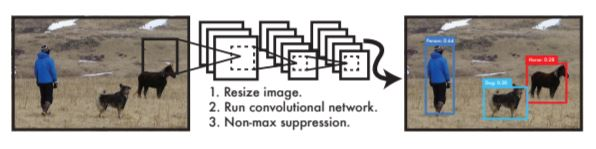
\includegraphics[width=0.7\textwidth]{chapter2/images/yolo.jpg}
    \caption{กระบวนการทำงานของโครงสร้างโมเดลปัญญาประดิษฐ์ของ YOLO}
    \label{fig:yolo}
\end{figure}

โครงสร้างโมเดลปัญญาประดิษฐ์ของ YOLO เป็นโครงสร้างที่มีความเร็วมาก มีความเร็วในการประมวลผลถึง 45 เฟรมต่อวิ ทำให้สามารถประมวลผลแบบเรียลไทม์ได้ นอกจากนั้นยังมีความแม่นยำ mAP มากกว่าโมเดลสำหรับตรวจจับวัตถุอื่นๆถึง 2 เท่า ซึ่งเหตุผลที่โครงสร้างโมเดลปัญญาประดิษฐ์ของ YOLO เร็วกว่าโมเดลปัญญาประดิษฐ์ตัวอื่นๆ เนื่องจาก มีแนวคิดที่ต่างออกไป คือ สำหรับการตรวจจับวัตถุในวิธีการก่อนหน้าจะใช้วิธีทำนายกรอบสี่เหลี่ยมก่อน แล้วจึงค่อยนำกรอบสี่เหลี่ยมไปทำนายว่าเป็นหมวดหมู่อะไร ซึ่ง YOLO มีวิธีการที่ต่างออกไป คือ ทำนายตำแหน่งของกรอบสี่เหลี่ยมและทำนายว่ากรอบสี่เหลี่ยมนั้นเป็นหมวดหมู่อะไรพร้อมกัน โดยใช้โครงข่ายประสาทแบบคอนโวลูชั่น ด้วยแนวคิดนี้จึงเป็นที่มาของชื่อ YOLO หรือ you only look once การมองแค่เพียงครั้งเดียว 
\subsection*{โครงสร้างของโมเดลปัญญาประดิษฐ์ของ YOLO} 
\begin{figure}[!ht]
    \centering
    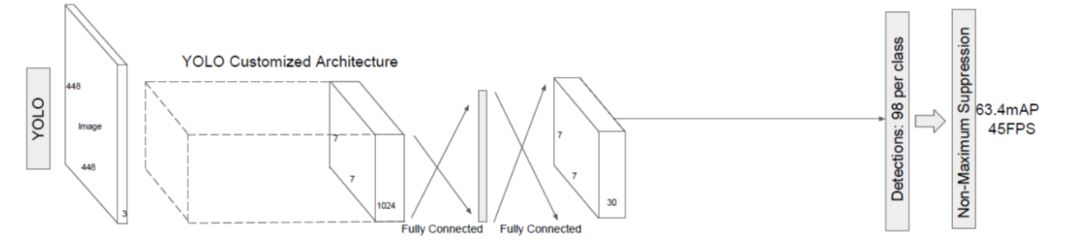
\includegraphics[width=0.7\textwidth]{chapter2/images/yolo_architecture.jpg}
    \caption{โครงสร้างทั่วไปของโมเดลปัญญาประดิษฐ์ของ YOLO}
    \label{fig:yolo_architecture}
\end{figure}

จากรูปภาพที่ \ref{fig:yolo_architecture} จะเห็นได้ว่า YOLO ใช้โครงข่ายประสาทเทียมเพียงตัวเดียวซึ่งภายในโครงข่ายจะมีกระบวนการหลักๆอยู่ 3 อย่าง กระบวนการแรกคือการสกัดคุณลักษณะกระบวนการนี้จะมีจำนวนชั้นของเลเยอร์ที่แตกต่างกันไปตามความลึกของการสกัดแล้วแต่โมเดล ซึ่งจะมีตัวอย่างอยู่ในบทความด้านล่าง และ ขั้นตอนถัดมา คือ การทำนายผล หลังจากที่ได้คุณลักษณะมาแล้วจะนำไปทำนายผลผ่าน Fully connected ซึ่งจะได้ผลลัพธ์ออกเป็นหมวดหมู่และตำแหน่งของกรอบสี่เหลี่ยม ขั้นตอนสุดท้ายคือ การทำ NMS เพื่อให้ได้ผลลัพธ์ที่ดีที่สุดออกมา



\par ซึ่งโครงสร้างโมเดลปัญญาประดิษฐ์ของ YOLO ที่ถูกใช้ในงานวิจัยนี้ประกอบไปด้วย 1) YOLOv3-tiny 2)YOLOv3 3) YOLOv3-spp	ซึ่งทั้ง 3 โครงสร้างจะมีความแตกต่างของโครงสร้างดังนี้
\begin{enumerate}
	\setlength\itemsep{-0.25em}
	\item YOLOv3-tiny ใช้ Max-Pooling layers ในขั้นตอนของการลดจำนวนข้อมูลตัวอย่าง
	\item YOLOv3 ใช้ Convolutional layers ในขั้นตอนของการลดจำนวนข้อมูลตัวอย่าง
	\item YOLOv3-spp ใช้ Convolutional layers+ฟีเจอร์ที่ดีที่สุดของ Max-Pooling layers ในขั้นตอนของการลดจำนวนข้อมูลตัวอย่าง
\end{enumerate}

\begin{figure}[!ht]
    \centering
    \begin{subfigure}[b]{0.3\textwidth}
        \centering
        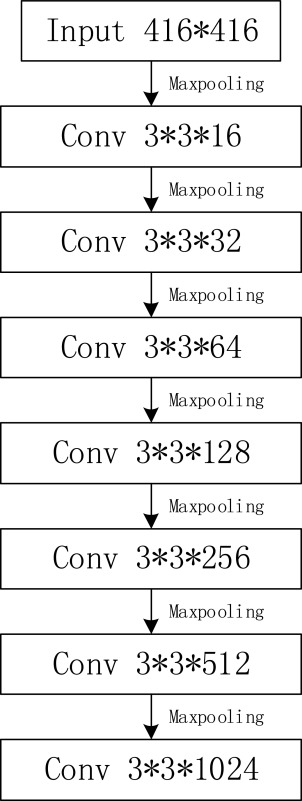
\includegraphics[width=\textwidth]{chapter2/images/yolo_tiny.jpg}
	 \caption{โครงสร้างโมเดลปัญญาประดิษฐ์ของ YOLOv3-tiny}
        \label{fig:tiny}
    \end{subfigure}
    \begin{subfigure}[b]{0.6\textwidth}
        \centering
        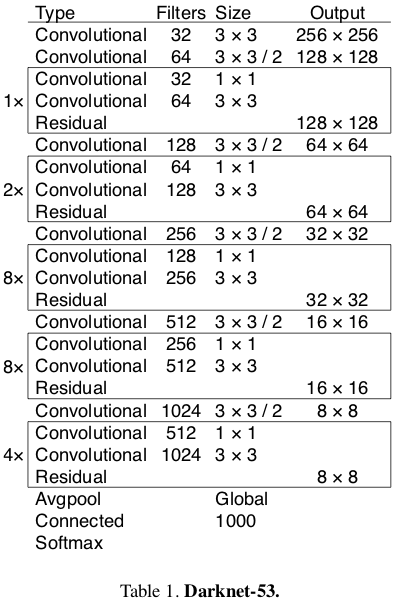
\includegraphics[width=\textwidth]{chapter2/images/yolo_darknet.png}
	 \caption{โครงสร้างโมเดลปัญญาประดิษฐ์ของ YOLOv3}
       \label{fig:darknet}
    \end{subfigure}
    \begin{subfigure}[b]{0.9\textwidth}
        \centering
        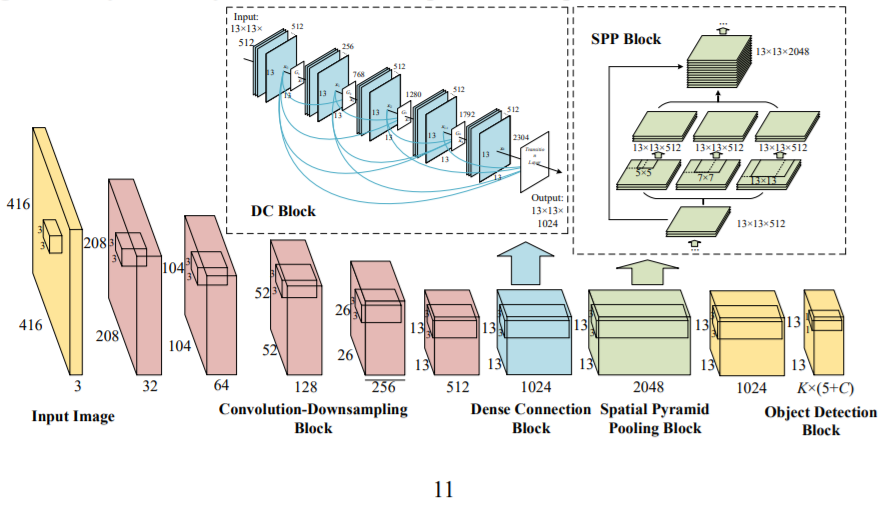
\includegraphics[width=\textwidth]{chapter2/images/yolo_spp.png}
	 \caption{โครงสร้างโมเดลปัญญาประดิษฐ์ของ YOLOv3-spp}
       \label{fig:spp}
    \end{subfigure}
    \caption{โครงสร้างโมเดลปัญญาประดิษฐ์ของ YOLO}
    \label{fig:yolo-architecture}
\end{figure}

